\section{Results}
\subsection{Survey results in summary}
\justify

%- Present results in the order of the research questions
%- Amount of records, amount of faulty records
%- Uncertainties
%- Present logically all results and interesting specific questions
%- Compare parking with original Travel Time Matrix values and values collected by me
%- Charts, statistics
%-Just show your findings, no nonsense
In this chapter we will discuss survey results which fit the criteria discussed in \hyperref[sec:processdata]{\fullref{sec:processdata}}. The survey received a total of 5579 visits from 4320 unique IP addresses. 848 unique IP addresses visited the survey more than one time and in total 1060 unique IP addresses sent data to the survey. 24.5 percent of all visitors submitted at least one data row. On average one respondent submitted 4.9 data rows. 

The survey received in total 5183 data rows. All postal code areas were represented in the survey results (figure~\ref{fig:postalvis_answers}), but the data row count histogram was heavily skewed to the right, with first quartile being 8 data rows, second (median) 17 data rows and third 42 data rows (table~\ref{tab:muns_answer_stats}). There were five postal code areas with more than one hundred data rows and 55 postal code areas with less than ten data rows. In \textit{postal} there are 167 postal code areas in Helsinki, Espoo, Vantaa, and Kauniainen combined.

\begin{hyphenrules}{nohyphenation}
    \begin{table}[H]
        \centering
        \def\arraystretch{1.2}
        \setlength\tabcolsep{4pt}
        \caption[Answer counts by municipality]{Amount of data rows received per municipality in Helsinki Capital Region.} 
        \label{tab:muns_answer_stats}
        \begin{tabular}{ @{} >{\raggedright\arraybackslash}p{3cm} >{\raggedright\arraybackslash}p{2cm} >{\raggedright\arraybackslash}p{4cm} >{\raggedright\arraybackslash}p{2cm} >{\raggedright\arraybackslash}p{2cm} @{} }
            \toprule
            Municipality & Data rows total & Most data rows in municipality & Mean & Median \\
            \midrule
            Helsinki & 3777 & 271 (00100 Helsinki Keskusta - Etu-Töölö) & 45.0 & 34.5 \\
            Espoo & 637 & 84 (02600 Etelä-Leppävaara) & 17.7 & 9.0 \\
            Vantaa & 746 & 91 (01510 Kirkonkylä-Veromäki) & 16.2 & 8.0 \\
            Kauniainen & 23 & 23 (02700 Kauniainen) & 23 & 23 \\
            % use \usepackage[table]{xcolor} and \usepackage{booktabs} to define \greyrule
            \greyrule
            All & 5183 & 271 (00100 Helsinki Keskusta - Etu-Töölö) & 31.0 & 17.0 \\
            \bottomrule
        \end{tabular}
    \end{table} 
\end{hyphenrules}

\begin{figure}[H]%
    \centering
    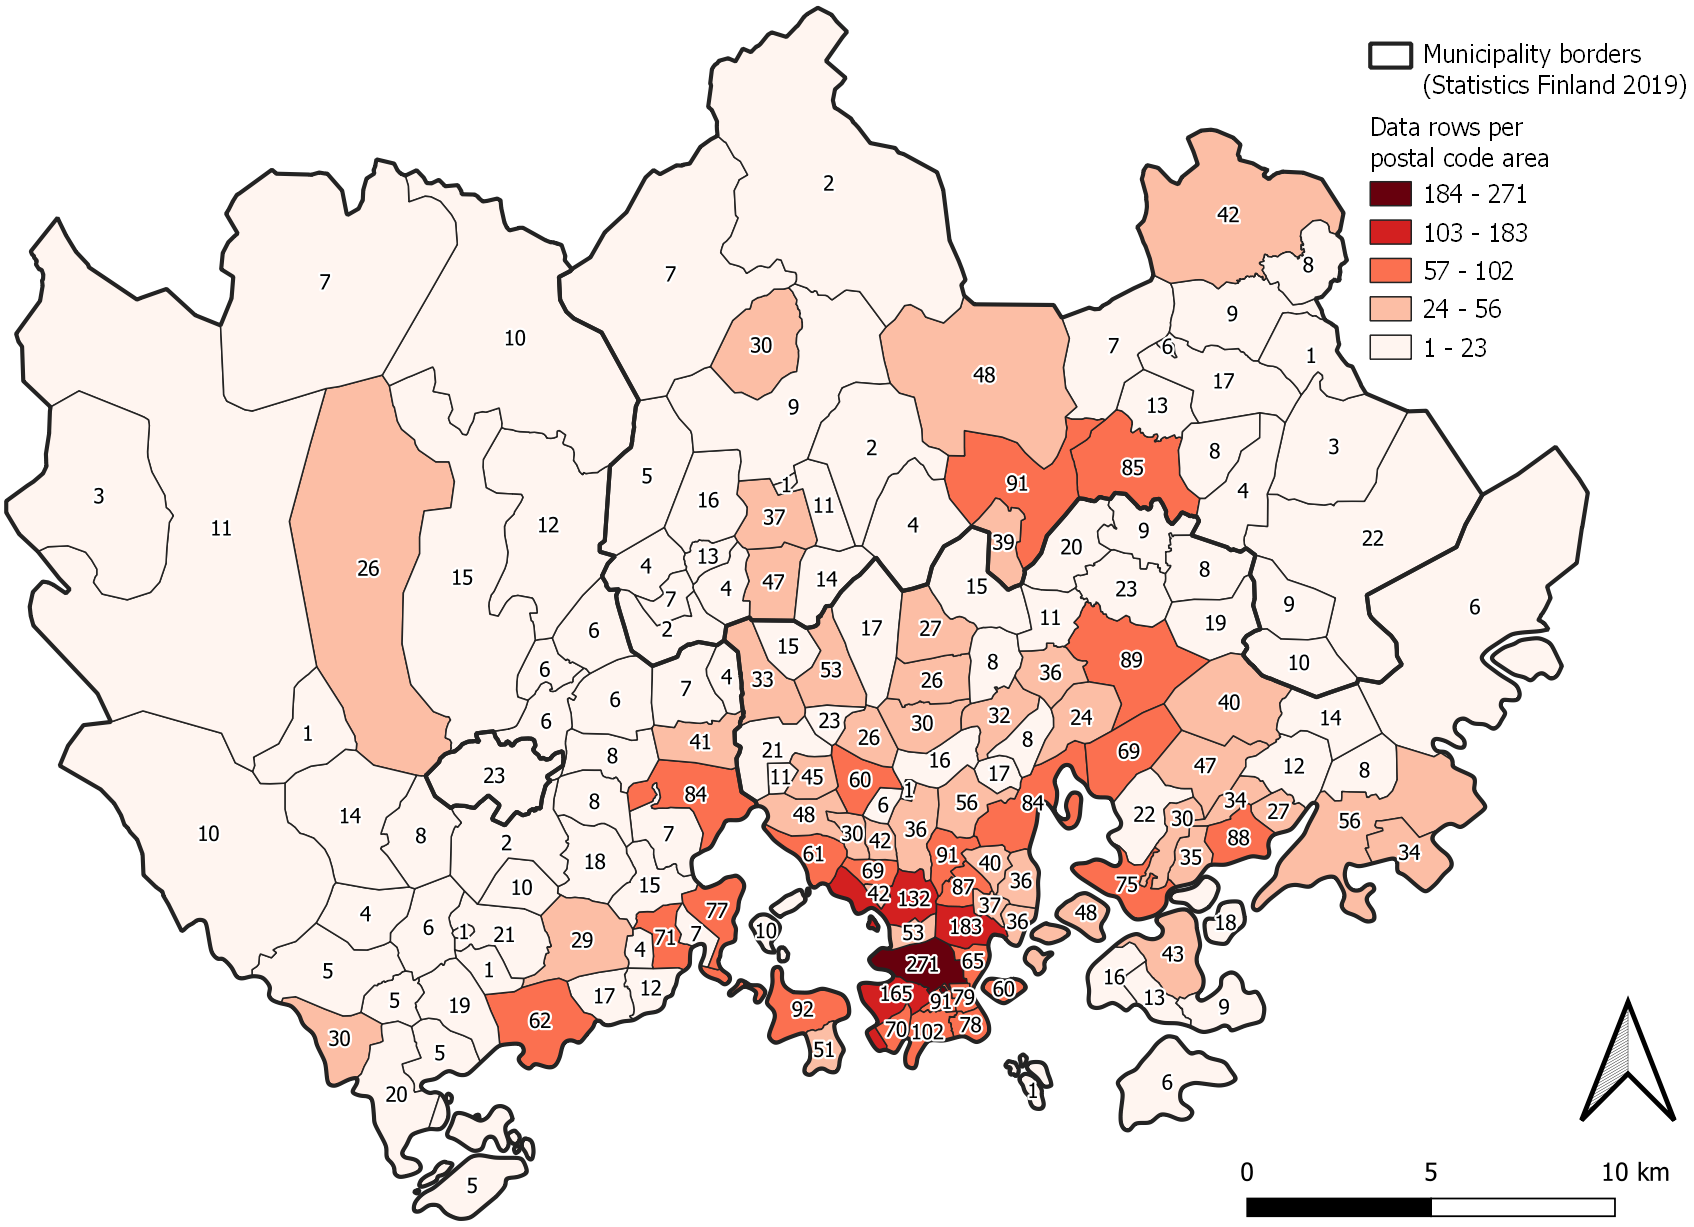
\includegraphics[width=.88\textwidth]{images/thesis_postalvis_answers.png}
    \caption[Data rows received per postal code area]{This figure illustrates the data rows received in the survey per postal code area. Classes are in natural breaks (Jenks). Municipality borders are based on \textit{postal} data.}%
    \label{fig:postalvis_answers}%
\end{figure}

\begin{figure}[H]%
    \centering
    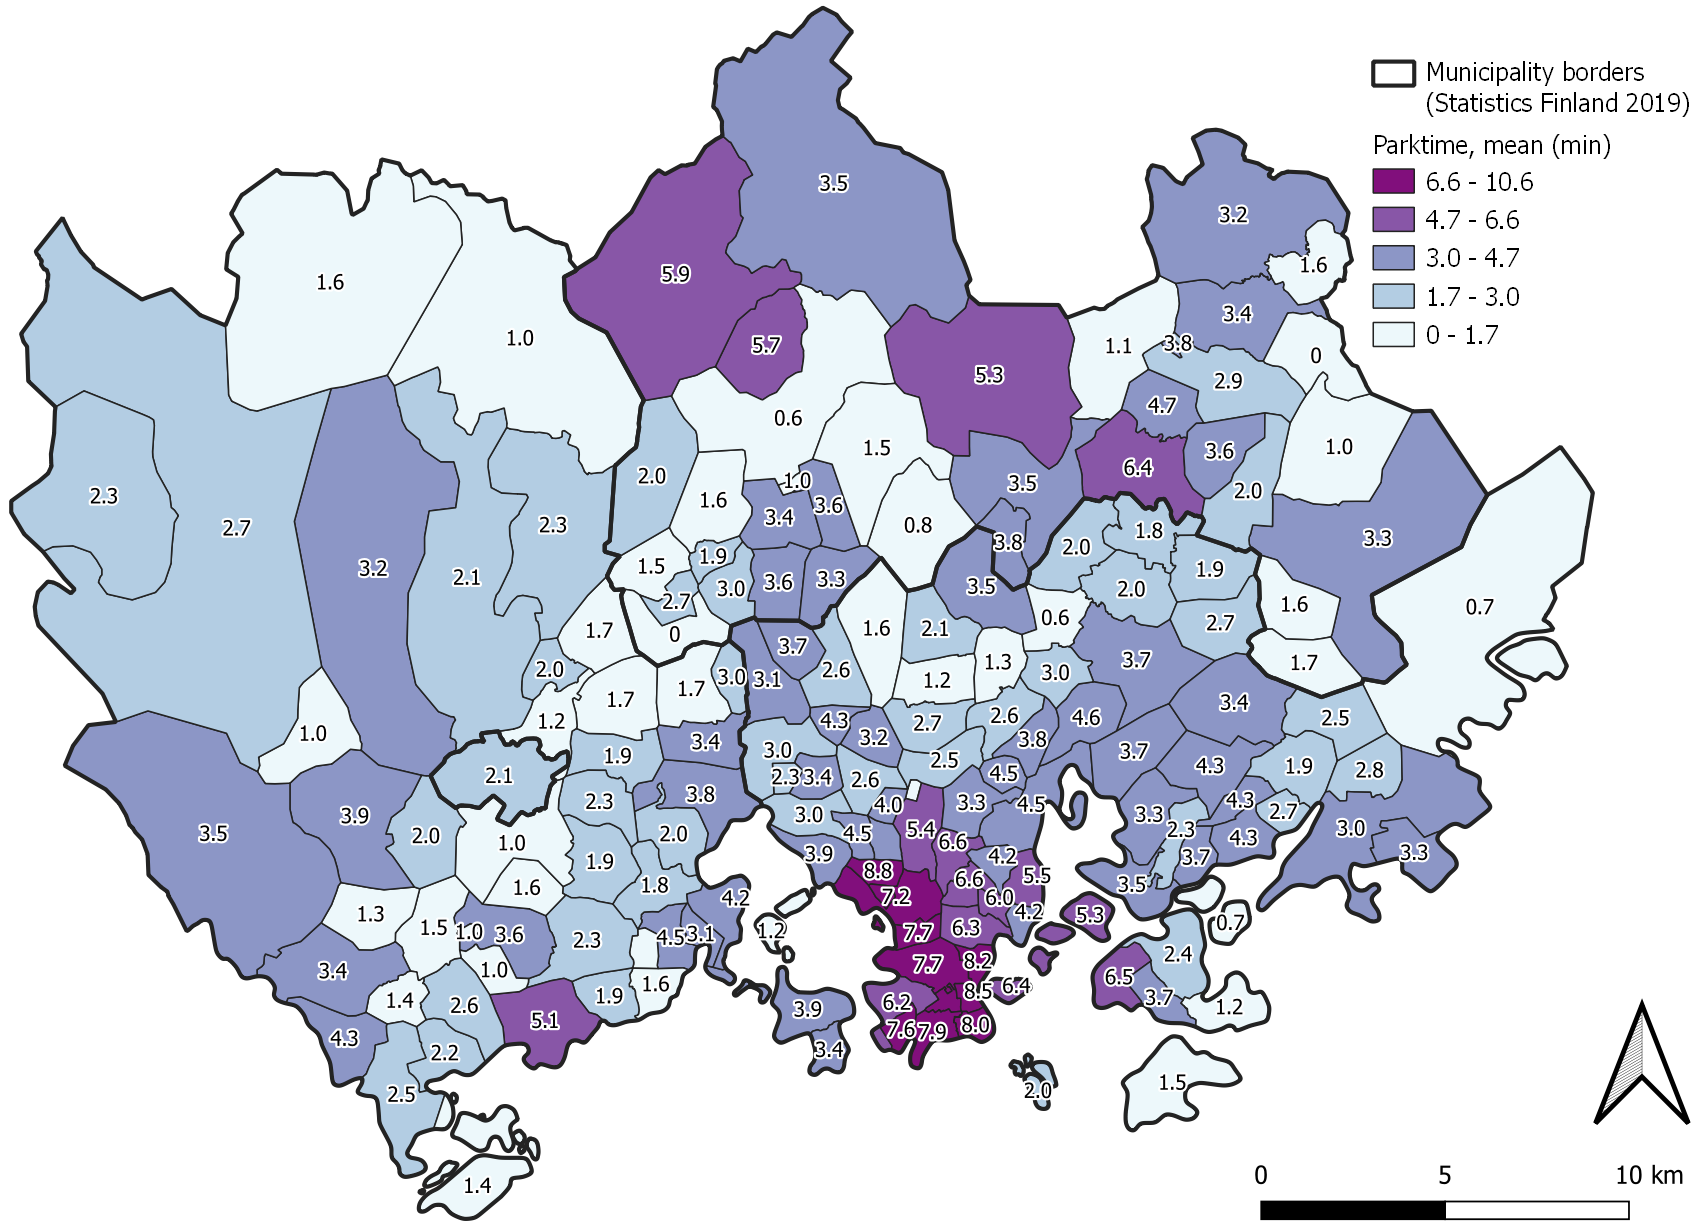
\includegraphics[width=.88\textwidth]{images/thesis_postalvis_parkmean.png}
    \caption[Parktime, mean, in the reseach area]{This figure illustrates the mean duration of searching for parking and parking one's car, usually, in each postal code area.}%
    \label{fig:postalvis_parkmean}%
\end{figure}

\begin{figure}[H]%
    \centering
    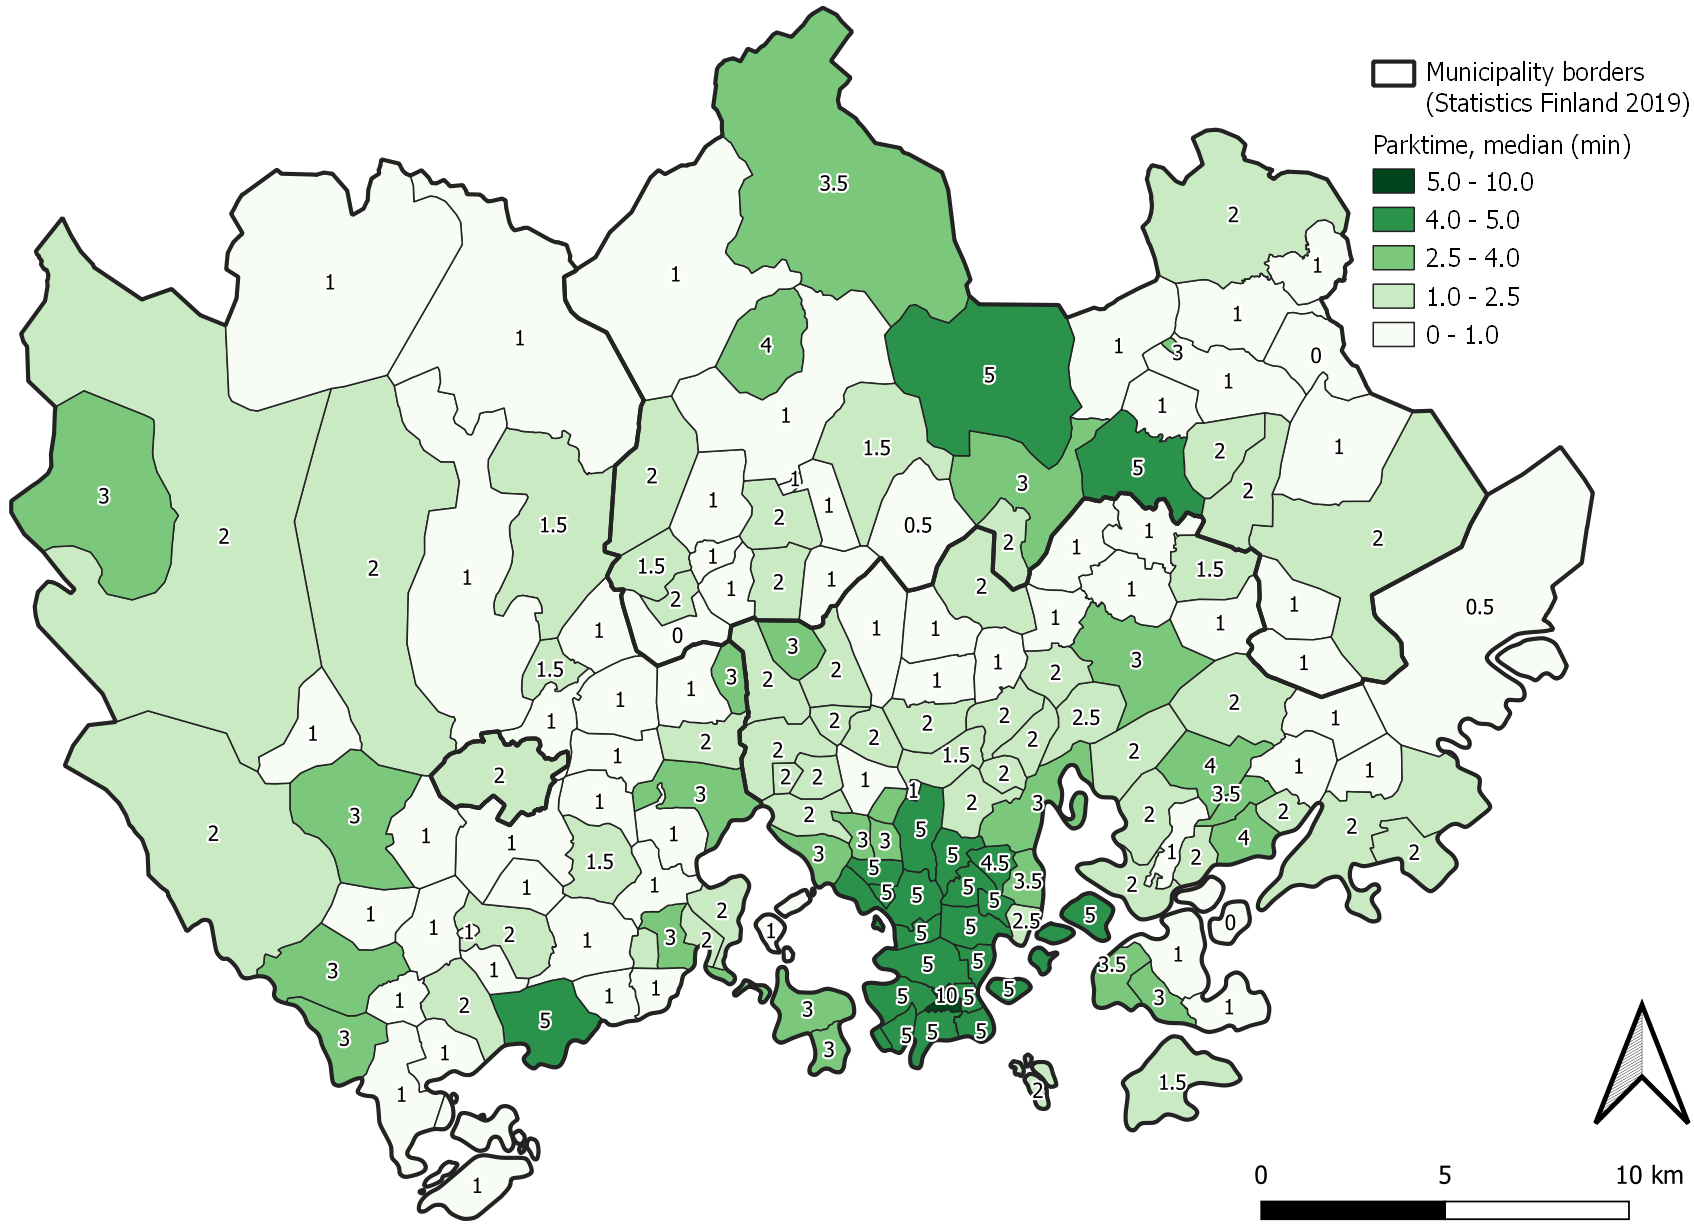
\includegraphics[width=.88\textwidth]{images/thesis_postalvis_parkmedian.png}
    \caption[Parktime, median, in the reseach area]{This figure illustrates the median duration of searching for parking and parking one's car, usually, in each postal code area.}%
    \label{fig:postalvis_parkmedian}%
\end{figure}

\begin{figure}[H]%
    \centering
    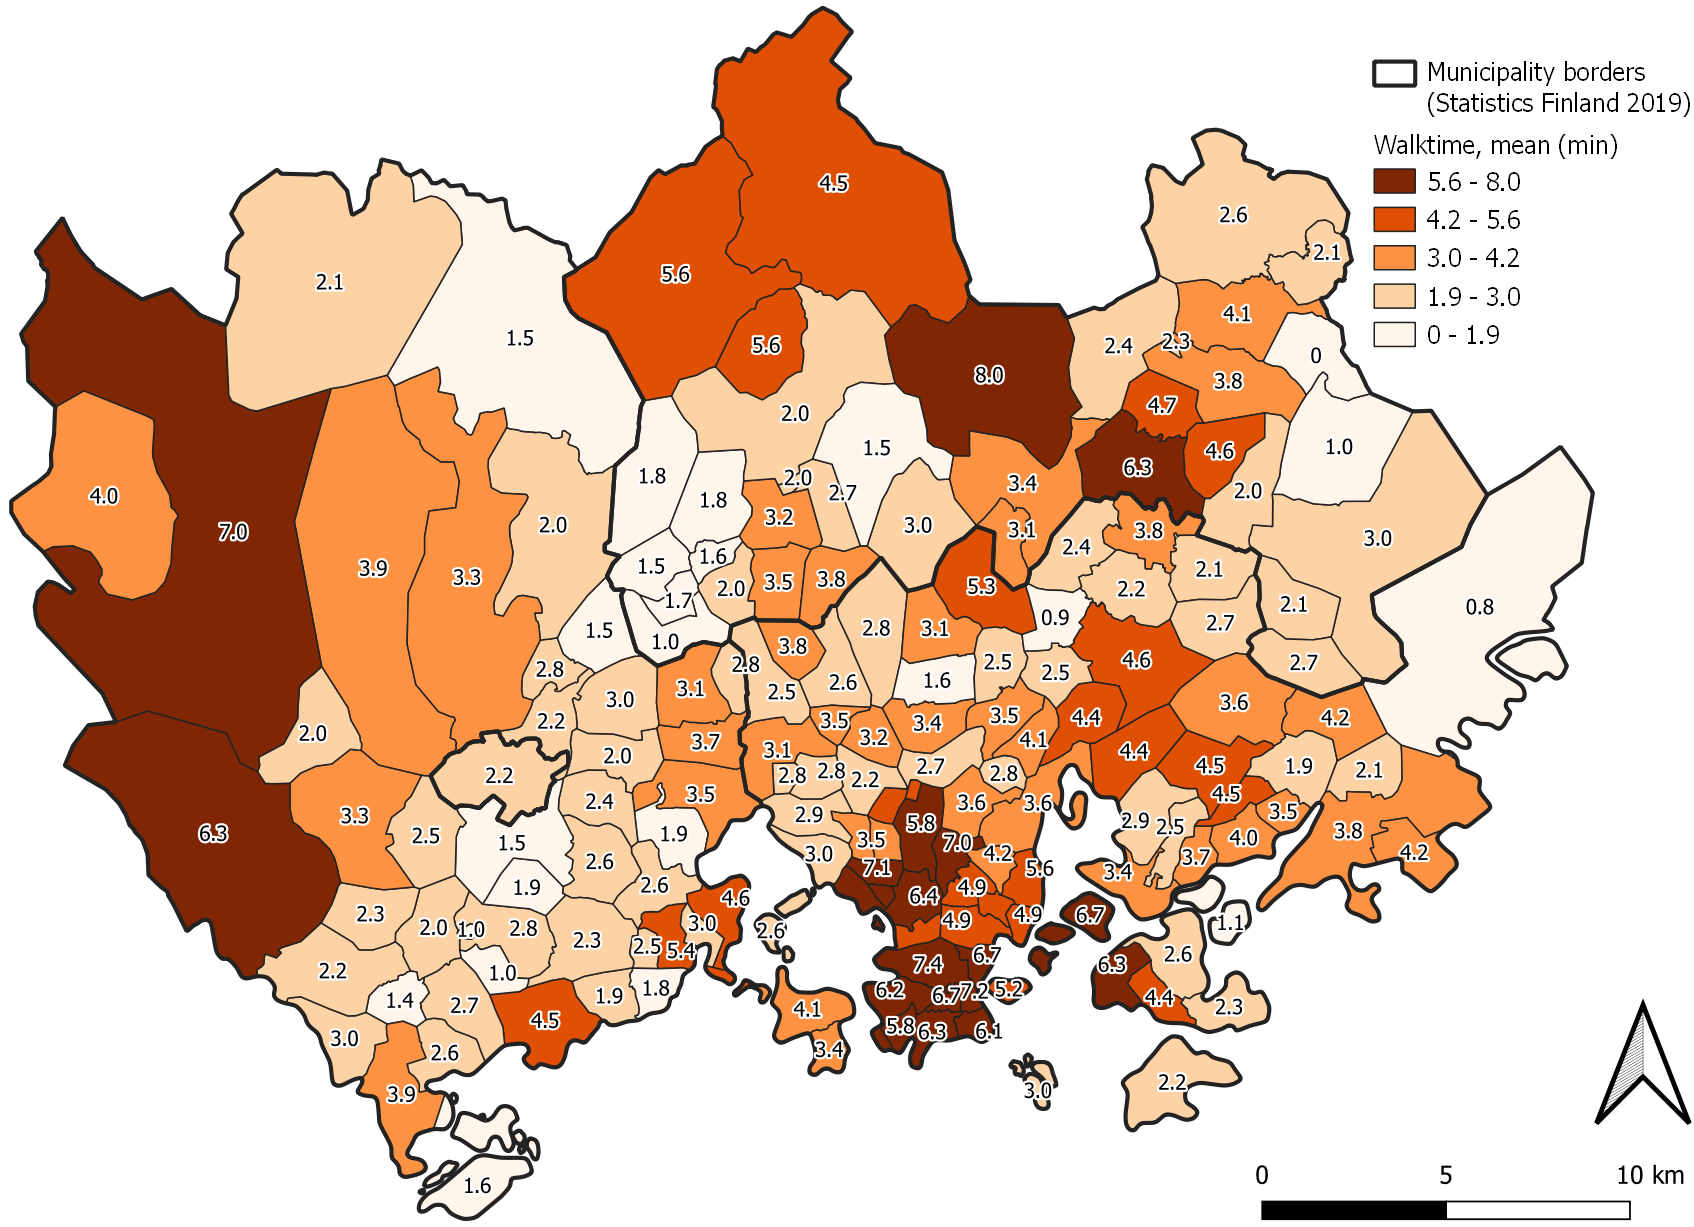
\includegraphics[width=.88\textwidth]{images/thesis_postalvis_walkmean.png}
    \caption[Walktime, mean, in the research area]{This figure illustrates the mean duration of walking from one's parked car to the final destination, usually, in each postal code area.}%
    \label{fig:postalvis_walkmean}%
\end{figure}

\begin{figure}[H]%
    \centering
    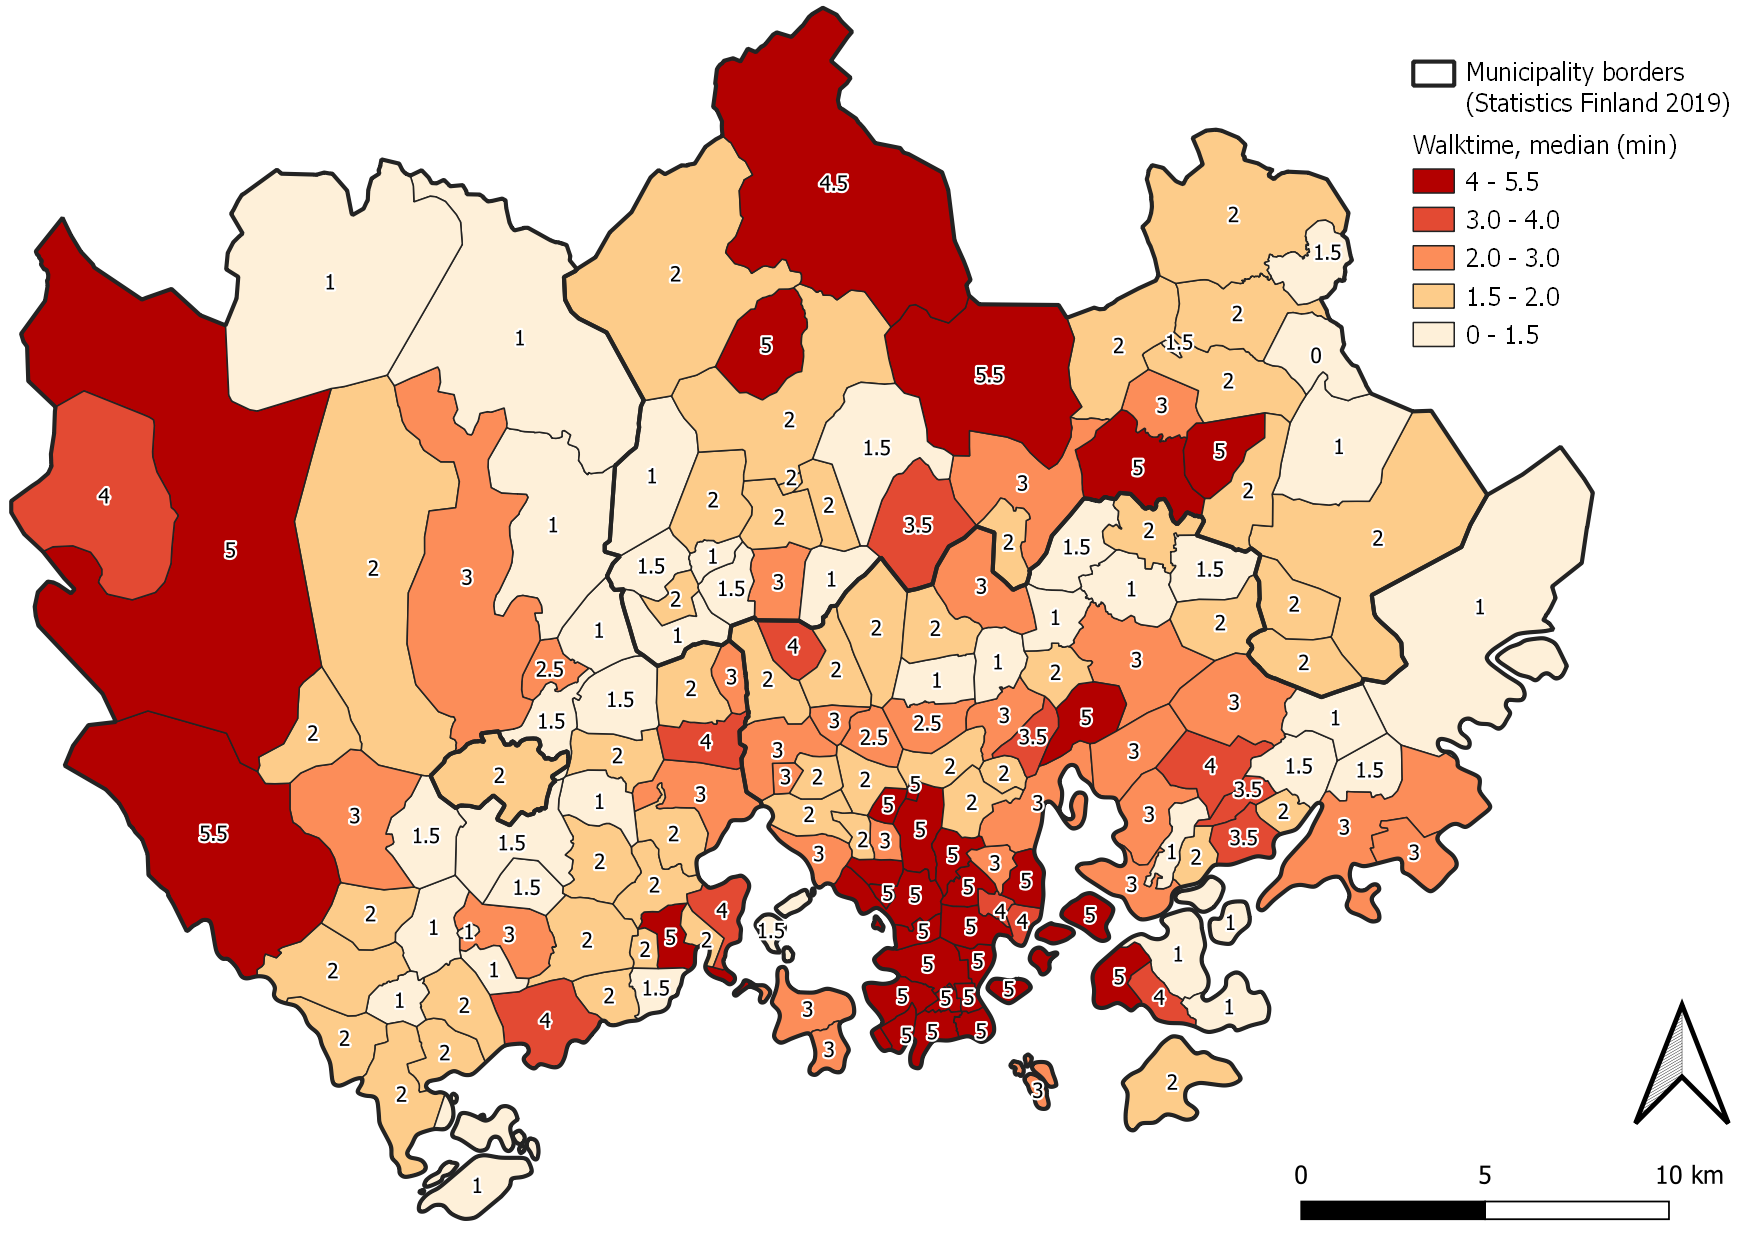
\includegraphics[width=.88\textwidth]{images/thesis_postalvis_walkmedian.png}
    \caption[Walktime, median, in the research area]{This figure illustrates the median duration of walking from one's parked car to the final destination, usually, in each postal code area.}%
    \label{fig:postalvis_walkmedian}%
\end{figure}

\textcolor{red}{Insert taulukko or teemakartta about answers (convey spatial distribution)}

\subsection{Statistics}
\justify

Preliminary findings
\begin{itemize}
    \item In total 5183 answers, 31.03 answers on average per postal code area. parktime\_mean 3.24min, walktime\_mean 3.40min
    \item Helsinki 3777 answers, on average 45.0 answers per postal code area. parktime\_mean 3.98min, walktime\_mean 3.95min
    \item Helsinki inner city ( 3777 answers, on average 45.0 answers per postal code area. parktime\_mean 3.98min, walktime\_mean 3.95min
    \item Espoo 746 answers, on average 17.7 answers per postal code area. parktime\_mean 2.73min, walktime\_mean 2.97min
    \item Vantaa 637 answers, on average 16.2 answers per postal code area. parktime\_mean 2.32min, walktime\_mean 2.78min
    \item Kauniainen 23 answers, parktime\_mean 2.13min, walktime\_mean 2.22min
\end{itemize}